\documentclass[1p]{elsarticle_modified}
%\bibliographystyle{elsarticle-num}

%\usepackage[colorlinks]{hyperref}
%\usepackage{abbrmath_seonhwa} %\Abb, \Ascr, \Acal ,\Abf, \Afrak
\usepackage{amsfonts}
\usepackage{amssymb}
\usepackage{amsmath}
\usepackage{amsthm}
\usepackage{scalefnt}
\usepackage{amsbsy}
\usepackage{kotex}
\usepackage{caption}
\usepackage{subfig}
\usepackage{color}
\usepackage{graphicx}
\usepackage{xcolor} %% white, black, red, green, blue, cyan, magenta, yellow
\usepackage{float}
\usepackage{setspace}
\usepackage{hyperref}

\usepackage{tikz}
\usetikzlibrary{arrows}

\usepackage{multirow}
\usepackage{array} % fixed length table
\usepackage{hhline}

%%%%%%%%%%%%%%%%%%%%%
\makeatletter
\renewcommand*\env@matrix[1][\arraystretch]{%
	\edef\arraystretch{#1}%
	\hskip -\arraycolsep
	\let\@ifnextchar\new@ifnextchar
	\array{*\c@MaxMatrixCols c}}
\makeatother %https://tex.stackexchange.com/questions/14071/how-can-i-increase-the-line-spacing-in-a-matrix
%%%%%%%%%%%%%%%

\usepackage[normalem]{ulem}

\newcommand{\msout}[1]{\ifmmode\text{\sout{\ensuremath{#1}}}\else\sout{#1}\fi}
%SOURCE: \msout is \stkout macro in https://tex.stackexchange.com/questions/20609/strikeout-in-math-mode

\newcommand{\cancel}[1]{
	\ifmmode
	{\color{red}\msout{#1}}
	\else
	{\color{red}\sout{#1}}
	\fi
}

\newcommand{\add}[1]{
	{\color{blue}\uwave{#1}}
}

\newcommand{\replace}[2]{
	\ifmmode
	{\color{red}\msout{#1}}{\color{blue}\uwave{#2}}
	\else
	{\color{red}\sout{#1}}{\color{blue}\uwave{#2}}
	\fi
}

\newcommand{\Sol}{\mathcal{S}} %segment
\newcommand{\D}{D} %diagram
\newcommand{\A}{\mathcal{A}} %arc


%%%%%%%%%%%%%%%%%%%%%%%%%%%%%5 test

\def\sl{\operatorname{\textup{SL}}(2,\Cbb)}
\def\psl{\operatorname{\textup{PSL}}(2,\Cbb)}
\def\quan{\mkern 1mu \triangleright \mkern 1mu}

\theoremstyle{definition}
\newtheorem{thm}{Theorem}[section]
\newtheorem{prop}[thm]{Proposition}
\newtheorem{lem}[thm]{Lemma}
\newtheorem{ques}[thm]{Question}
\newtheorem{cor}[thm]{Corollary}
\newtheorem{defn}[thm]{Definition}
\newtheorem{exam}[thm]{Example}
\newtheorem{rmk}[thm]{Remark}
\newtheorem{alg}[thm]{Algorithm}

\newcommand{\I}{\sqrt{-1}}
\begin{document}

%\begin{frontmatter}
%
%\title{Boundary parabolic representations of knots up to 8 crossings}
%
%%% Group authors per affiliation:
%\author{Yunhi Cho} 
%\address{Department of Mathematics, University of Seoul, Seoul, Korea}
%\ead{yhcho@uos.ac.kr}
%
%
%\author{Seonhwa Kim} %\fnref{s_kim}}
%\address{Center for Geometry and Physics, Institute for Basic Science, Pohang, 37673, Korea}
%\ead{ryeona17@ibs.re.kr}
%
%\author{Hyuk Kim}
%\address{Department of Mathematical Sciences, Seoul National University, Seoul 08826, Korea}
%\ead{hyukkim@snu.ac.kr}
%
%\author{Seokbeom Yoon}
%\address{Department of Mathematical Sciences, Seoul National University, Seoul, 08826,  Korea}
%\ead{sbyoon15@snu.ac.kr}
%
%\begin{abstract}
%We find all boundary parabolic representation of knots up to 8 crossings.
%
%\end{abstract}
%\begin{keyword}
%    \MSC[2010] 57M25 
%\end{keyword}
%
%\end{frontmatter}

%\linenumbers
%\tableofcontents
%
\newcommand\colored[1]{\textcolor{white}{\rule[-0.35ex]{0.8em}{1.4ex}}\kern-0.8em\color{red} #1}%
%\newcommand\colored[1]{\textcolor{white}{ #1}\kern-2.17ex	\textcolor{white}{ #1}\kern-1.81ex	\textcolor{white}{ #1}\kern-2.15ex\color{red}#1	}

{\Large $\underline{12n_{0107}~(K12n_{0107})}$}

\setlength{\tabcolsep}{10pt}
\renewcommand{\arraystretch}{1.6}
\vspace{1cm}\begin{tabular}{m{100pt}>{\centering\arraybackslash}m{274pt}}
\multirow{5}{120pt}{
	\centering
	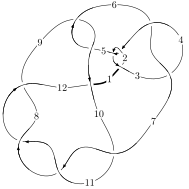
\includegraphics[width=112pt]{../../../GIT/diagram.site/Diagrams/png/2196_12n_0107.png}\\
\ \ \ A knot diagram\footnotemark}&
\allowdisplaybreaks
\textbf{Linearized knot diagam} \\
\cline{2-2}
 &
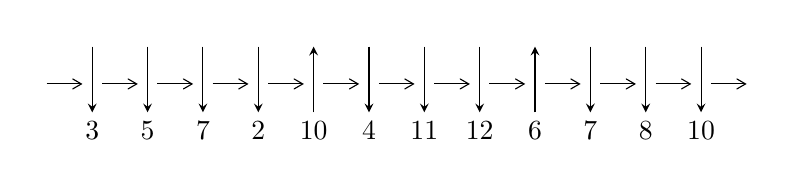
\begin{tikzpicture}[x=20pt, y=17pt]
	% nodes
	\node (C0) at (0, 0) {};
	\node (C1) at (1, 0) {};
	\node (C1U) at (1, +1) {};
	\node (C1D) at (1, -1) {3};

	\node (C2) at (2, 0) {};
	\node (C2U) at (2, +1) {};
	\node (C2D) at (2, -1) {5};

	\node (C3) at (3, 0) {};
	\node (C3U) at (3, +1) {};
	\node (C3D) at (3, -1) {7};

	\node (C4) at (4, 0) {};
	\node (C4U) at (4, +1) {};
	\node (C4D) at (4, -1) {2};

	\node (C5) at (5, 0) {};
	\node (C5U) at (5, +1) {};
	\node (C5D) at (5, -1) {10};

	\node (C6) at (6, 0) {};
	\node (C6U) at (6, +1) {};
	\node (C6D) at (6, -1) {4};

	\node (C7) at (7, 0) {};
	\node (C7U) at (7, +1) {};
	\node (C7D) at (7, -1) {11};

	\node (C8) at (8, 0) {};
	\node (C8U) at (8, +1) {};
	\node (C8D) at (8, -1) {12};

	\node (C9) at (9, 0) {};
	\node (C9U) at (9, +1) {};
	\node (C9D) at (9, -1) {6};

	\node (C10) at (10, 0) {};
	\node (C10U) at (10, +1) {};
	\node (C10D) at (10, -1) {7};

	\node (C11) at (11, 0) {};
	\node (C11U) at (11, +1) {};
	\node (C11D) at (11, -1) {8};

	\node (C12) at (12, 0) {};
	\node (C12U) at (12, +1) {};
	\node (C12D) at (12, -1) {10};
	\node (C13) at (13, 0) {};

	% arrows
	\draw[->,>={angle 60}]
	(C0) edge (C1) (C1) edge (C2) (C2) edge (C3) (C3) edge (C4) (C4) edge (C5) (C5) edge (C6) (C6) edge (C7) (C7) edge (C8) (C8) edge (C9) (C9) edge (C10) (C10) edge (C11) (C11) edge (C12) (C12) edge (C13) ;	\draw[->,>=stealth]
	(C1U) edge (C1D) (C2U) edge (C2D) (C3U) edge (C3D) (C4U) edge (C4D) (C5D) edge (C5U) (C6U) edge (C6D) (C7U) edge (C7D) (C8U) edge (C8D) (C9D) edge (C9U) (C10U) edge (C10D) (C11U) edge (C11D) (C12U) edge (C12D) ;
	\end{tikzpicture} \\
\hhline{~~} \\& 
\textbf{Solving Sequence} \\ \cline{2-2} 
 &
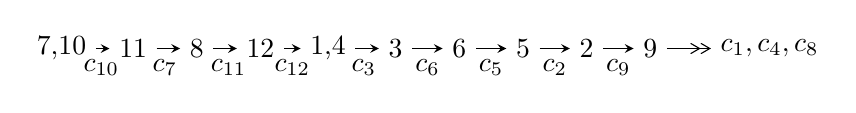
\begin{tikzpicture}[x=23pt, y=7pt]
	% node
	\node (A0) at (-1/8, 0) {7,10};
	\node (A1) at (1, 0) {11};
	\node (A2) at (2, 0) {8};
	\node (A3) at (3, 0) {12};
	\node (A4) at (65/16, 0) {1,4};
	\node (A5) at (41/8, 0) {3};
	\node (A6) at (49/8, 0) {6};
	\node (A7) at (57/8, 0) {5};
	\node (A8) at (65/8, 0) {2};
	\node (A9) at (73/8, 0) {9};
	\node (C1) at (1/2, -1) {$c_{10}$};
	\node (C2) at (3/2, -1) {$c_{7}$};
	\node (C3) at (5/2, -1) {$c_{11}$};
	\node (C4) at (7/2, -1) {$c_{12}$};
	\node (C5) at (37/8, -1) {$c_{3}$};
	\node (C6) at (45/8, -1) {$c_{6}$};
	\node (C7) at (53/8, -1) {$c_{5}$};
	\node (C8) at (61/8, -1) {$c_{2}$};
	\node (C9) at (69/8, -1) {$c_{9}$};
	\node (A10) at (11, 0) {$c_{1},c_{4},c_{8}$};

	% edge
	\draw[->,>=stealth]	
	(A0) edge (A1) (A1) edge (A2) (A2) edge (A3) (A3) edge (A4) (A4) edge (A5) (A5) edge (A6) (A6) edge (A7) (A7) edge (A8) (A8) edge (A9) ;
	\draw[->>,>={angle 60}]	
	(A9) edge (A10);
\end{tikzpicture} \\ 

\end{tabular} \\

\footnotetext{
The image of knot diagram is generated by the software ``\textbf{Draw programme}" developed by Andrew Bartholomew(\url{http://www.layer8.co.uk/maths/draw/index.htm\#Running-draw}), where we modified some parts for our purpose(\url{https://github.com/CATsTAILs/LinksPainter}).
}\phantom \\ \newline 
\centering \textbf{Ideals for irreducible components\footnotemark of $X_{\text{par}}$} 
 
\begin{align*}
I^u_{1}&=\langle 
47441368 u^{25}+57693789 u^{24}+\cdots+104373924 b+18568285,\\
\phantom{I^u_{1}}&\phantom{= \langle  }120201295 u^{25}+398061213 u^{24}+\cdots+104373924 a+783424087,\;u^{26}+5 u^{25}+\cdots+14 u-1\rangle \\
I^u_{2}&=\langle 
2 a^2 u+a^2- a u+b- a+2 u,\;a^3- a^2 u+a^2-2 a u+4 a-2 u+3,\;u^2- u-1\rangle \\
I^u_{3}&=\langle 
b+1,\;a,\;u+1\rangle \\
\\
\end{align*}
\raggedright * 3 irreducible components of $\dim_{\mathbb{C}}=0$, with total 33 representations.\\
\footnotetext{All coefficients of polynomials are rational numbers. But the coefficients are sometimes approximated in decimal forms when there is not enough margin.}
\newpage
\renewcommand{\arraystretch}{1}
\centering \section*{I. $I^u_{1}= \langle 4.74\times10^{7} u^{25}+5.77\times10^{7} u^{24}+\cdots+1.04\times10^{8} b+1.86\times10^{7},\;1.20\times10^{8} u^{25}+3.98\times10^{8} u^{24}+\cdots+1.04\times10^{8} a+7.83\times10^{8},\;u^{26}+5 u^{25}+\cdots+14 u-1 \rangle$}
\flushleft \textbf{(i) Arc colorings}\\
\begin{tabular}{m{7pt} m{180pt} m{7pt} m{180pt} }
\flushright $a_{7}=$&$\begin{pmatrix}0\\u\end{pmatrix}$ \\
\flushright $a_{10}=$&$\begin{pmatrix}1\\0\end{pmatrix}$ \\
\flushright $a_{11}=$&$\begin{pmatrix}1\\u^2\end{pmatrix}$ \\
\flushright $a_{8}=$&$\begin{pmatrix}- u\\- u^3+u\end{pmatrix}$ \\
\flushright $a_{12}=$&$\begin{pmatrix}- u^2+1\\- u^4+2 u^2\end{pmatrix}$ \\
\flushright $a_{1}=$&$\begin{pmatrix}u^4-3 u^2+1\\- u^4+2 u^2\end{pmatrix}$ \\
\flushright $a_{4}=$&$\begin{pmatrix}-1.15164 u^{25}-3.81380 u^{24}+\cdots-24.4464 u-7.50594\\-0.454533 u^{25}-0.552761 u^{24}+\cdots+13.0629 u-0.177902\end{pmatrix}$ \\
\flushright $a_{3}=$&$\begin{pmatrix}-1.15164 u^{25}-3.81380 u^{24}+\cdots-24.4464 u-7.50594\\3.33329 u^{25}+11.3654 u^{24}+\cdots+41.4363 u-2.12231\end{pmatrix}$ \\
\flushright $a_{6}=$&$\begin{pmatrix}-0.633480 u^{25}-1.36564 u^{24}+\cdots+2.69053 u+4.69952\\-1.23184 u^{25}-3.55184 u^{24}+\cdots-6.61306 u+0.205455\end{pmatrix}$ \\
\flushright $a_{5}=$&$\begin{pmatrix}0.598359 u^{25}+2.18620 u^{24}+\cdots+9.30359 u+4.49406\\-1.23184 u^{25}-3.55184 u^{24}+\cdots-6.61306 u+0.205455\end{pmatrix}$ \\
\flushright $a_{2}=$&$\begin{pmatrix}-0.598359 u^{25}-2.18620 u^{24}+\cdots-9.30359 u-4.49406\\-0.203032 u^{25}+0.469119 u^{24}+\cdots+15.6624 u-0.533217\end{pmatrix}$ \\
\flushright $a_{9}=$&$\begin{pmatrix}u^3-2 u\\u^5-3 u^3+u\end{pmatrix}$\\&\end{tabular}
\flushleft \textbf{(ii) Obstruction class $= -1$}\\~\\
\flushleft \textbf{(iii) Cusp Shapes $= -\frac{92088909}{17395654} u^{25}-\frac{188693588}{8697827} u^{24}+\cdots-\frac{885802456}{8697827} u-\frac{15795407}{8697827}$}\\~\\
\newpage\renewcommand{\arraystretch}{1}
\flushleft \textbf{(iv) u-Polynomials at the component}\newline \\
\begin{tabular}{m{50pt}|m{274pt}}
Crossings & \hspace{64pt}u-Polynomials at each crossing \\
\hline $$\begin{aligned}c_{1}\end{aligned}$$&$\begin{aligned}
&u^{26}+20 u^{25}+\cdots+79 u+1
\end{aligned}$\\
\hline $$\begin{aligned}c_{2},c_{4}\end{aligned}$$&$\begin{aligned}
&u^{26}-4 u^{25}+\cdots-11 u-1
\end{aligned}$\\
\hline $$\begin{aligned}c_{3},c_{6}\end{aligned}$$&$\begin{aligned}
&u^{26}-3 u^{25}+\cdots-6 u+2
\end{aligned}$\\
\hline $$\begin{aligned}c_{5},c_{9}\end{aligned}$$&$\begin{aligned}
&u^{26}-2 u^{25}+\cdots-96 u+64
\end{aligned}$\\
\hline $$\begin{aligned}c_{7},c_{8},c_{10}\\c_{11}\end{aligned}$$&$\begin{aligned}
&u^{26}+5 u^{25}+\cdots+14 u-1
\end{aligned}$\\
\hline $$\begin{aligned}c_{12}\end{aligned}$$&$\begin{aligned}
&u^{26}-21 u^{25}+\cdots+52120 u+337
\end{aligned}$\\
\hline
\end{tabular}\\~\\
\newpage\renewcommand{\arraystretch}{1}
\flushleft \textbf{(v) Riley Polynomials at the component}\newline \\
\begin{tabular}{m{50pt}|m{274pt}}
Crossings & \hspace{64pt}Riley Polynomials at each crossing \\
\hline $$\begin{aligned}c_{1}\end{aligned}$$&$\begin{aligned}
&y^{26}-24 y^{25}+\cdots-6127 y+1
\end{aligned}$\\
\hline $$\begin{aligned}c_{2},c_{4}\end{aligned}$$&$\begin{aligned}
&y^{26}-20 y^{25}+\cdots-79 y+1
\end{aligned}$\\
\hline $$\begin{aligned}c_{3},c_{6}\end{aligned}$$&$\begin{aligned}
&y^{26}-3 y^{25}+\cdots-40 y+4
\end{aligned}$\\
\hline $$\begin{aligned}c_{5},c_{9}\end{aligned}$$&$\begin{aligned}
&y^{26}+34 y^{25}+\cdots-95232 y+4096
\end{aligned}$\\
\hline $$\begin{aligned}c_{7},c_{8},c_{10}\\c_{11}\end{aligned}$$&$\begin{aligned}
&y^{26}-39 y^{25}+\cdots-304 y+1
\end{aligned}$\\
\hline $$\begin{aligned}c_{12}\end{aligned}$$&$\begin{aligned}
&y^{26}-123 y^{25}+\cdots-2285596764 y+113569
\end{aligned}$\\
\hline
\end{tabular}\\~\\
\newpage\flushleft \textbf{(vi) Complex Volumes and Cusp Shapes}
$$\begin{array}{c|c|c}  
\text{Solutions to }I^u_{1}& \I (\text{vol} + \sqrt{-1}CS) & \text{Cusp shape}\\
 \hline 
\begin{aligned}
u &= -0.476607 + 0.919429 I \\
a &= -0.688440 - 0.733293 I \\
b &= \phantom{-}0.227587 + 1.287750 I\end{aligned}
 & -5.18299 + 2.95142 I & -14.7696 - 4.0162 I \\ \hline\begin{aligned}
u &= -0.476607 - 0.919429 I \\
a &= -0.688440 + 0.733293 I \\
b &= \phantom{-}0.227587 - 1.287750 I\end{aligned}
 & -5.18299 - 2.95142 I & -14.7696 + 4.0162 I \\ \hline\begin{aligned}
u &= -0.757036\phantom{ +0.000000I} \\
a &= -0.441343\phantom{ +0.000000I} \\
b &= \phantom{-}0.637723\phantom{ +0.000000I}\end{aligned}
 & -1.34161\phantom{ +0.000000I} & -6.51520\phantom{ +0.000000I} \\ \hline\begin{aligned}
u &= \phantom{-}1.223650 + 0.232594 I \\
a &= -0.924838 - 0.484695 I \\
b &= \phantom{-}0.280314 - 1.358420 I\end{aligned}
 & -5.77000 - 3.25214 I & -11.73752 + 3.41900 I \\ \hline\begin{aligned}
u &= \phantom{-}1.223650 - 0.232594 I \\
a &= -0.924838 + 0.484695 I \\
b &= \phantom{-}0.280314 + 1.358420 I\end{aligned}
 & -5.77000 + 3.25214 I & -11.73752 - 3.41900 I \\ \hline\begin{aligned}
u &= -1.329480 + 0.241157 I \\
a &= \phantom{-}0.277950 + 0.611388 I \\
b &= \phantom{-}0.308061 + 0.000558 I\end{aligned}
 & -3.29395 - 1.34186 I & -11.30499 + 4.69401 I \\ \hline\begin{aligned}
u &= -1.329480 - 0.241157 I \\
a &= \phantom{-}0.277950 - 0.611388 I \\
b &= \phantom{-}0.308061 - 0.000558 I\end{aligned}
 & -3.29395 + 1.34186 I & -11.30499 - 4.69401 I \\ \hline\begin{aligned}
u &= \phantom{-}1.369250 + 0.095489 I \\
a &= \phantom{-}0.500507 - 0.680570 I \\
b &= \phantom{-}0.10931 - 1.70719 I\end{aligned}
 & -9.37037 - 1.40410 I & -14.8448 + 0.4920 I \\ \hline\begin{aligned}
u &= \phantom{-}1.369250 - 0.095489 I \\
a &= \phantom{-}0.500507 + 0.680570 I \\
b &= \phantom{-}0.10931 + 1.70719 I\end{aligned}
 & -9.37037 + 1.40410 I & -14.8448 - 0.4920 I \\ \hline\begin{aligned}
u &= \phantom{-}1.273730 + 0.536724 I \\
a &= \phantom{-}0.988931 + 0.204426 I \\
b &= -0.48656 + 1.60886 I\end{aligned}
 & -10.60190 - 7.95034 I & -14.2939 + 5.5201 I\\
 \hline 
 \end{array}$$\newpage$$\begin{array}{c|c|c}  
\text{Solutions to }I^u_{1}& \I (\text{vol} + \sqrt{-1}CS) & \text{Cusp shape}\\
 \hline 
\begin{aligned}
u &= \phantom{-}1.273730 - 0.536724 I \\
a &= \phantom{-}0.988931 - 0.204426 I \\
b &= -0.48656 - 1.60886 I\end{aligned}
 & -10.60190 + 7.95034 I & -14.2939 - 5.5201 I \\ \hline\begin{aligned}
u &= -0.586682 + 0.167108 I \\
a &= -0.045237 - 0.711969 I \\
b &= -0.71246 - 2.34576 I\end{aligned}
 & -2.72200 + 0.36882 I & -3.94523 + 10.24837 I \\ \hline\begin{aligned}
u &= -0.586682 - 0.167108 I \\
a &= -0.045237 + 0.711969 I \\
b &= -0.71246 + 2.34576 I\end{aligned}
 & -2.72200 - 0.36882 I & -3.94523 - 10.24837 I \\ \hline\begin{aligned}
u &= -0.348677 + 0.367916 I \\
a &= \phantom{-}1.247060 + 0.371784 I \\
b &= -0.209352 - 0.864493 I\end{aligned}
 & -0.636376 + 1.127340 I & -7.20662 - 6.11077 I \\ \hline\begin{aligned}
u &= -0.348677 - 0.367916 I \\
a &= \phantom{-}1.247060 - 0.371784 I \\
b &= -0.209352 + 0.864493 I\end{aligned}
 & -0.636376 - 1.127340 I & -7.20662 + 6.11077 I \\ \hline\begin{aligned}
u &= \phantom{-}0.424219 + 0.095685 I \\
a &= \phantom{-}0.07818 + 2.89428 I \\
b &= -0.1185550 - 0.0289313 I\end{aligned}
 & \phantom{-}2.35620 + 2.67700 I & \phantom{-}3.89989 + 1.35809 I \\ \hline\begin{aligned}
u &= \phantom{-}0.424219 - 0.095685 I \\
a &= \phantom{-}0.07818 - 2.89428 I \\
b &= -0.1185550 + 0.0289313 I\end{aligned}
 & \phantom{-}2.35620 - 2.67700 I & \phantom{-}3.89989 - 1.35809 I \\ \hline\begin{aligned}
u &= \phantom{-}1.63681\phantom{ +0.000000I} \\
a &= \phantom{-}0.377195\phantom{ +0.000000I} \\
b &= -1.87474\phantom{ +0.000000I}\end{aligned}
 & -9.79249\phantom{ +0.000000I} & \phantom{-}1.55260\phantom{ +0.000000I} \\ \hline\begin{aligned}
u &= -1.80599 + 0.06787 I \\
a &= \phantom{-}0.735548 - 0.651435 I \\
b &= -0.23521 - 1.59914 I\end{aligned}
 & -16.9214 + 4.6752 I & \phantom{-0.000000 } 0 \\ \hline\begin{aligned}
u &= -1.80599 - 0.06787 I \\
a &= \phantom{-}0.735548 + 0.651435 I \\
b &= -0.23521 + 1.59914 I\end{aligned}
 & -16.9214 - 4.6752 I & \phantom{-0.000000 } 0\\
 \hline 
 \end{array}$$\newpage$$\begin{array}{c|c|c}  
\text{Solutions to }I^u_{1}& \I (\text{vol} + \sqrt{-1}CS) & \text{Cusp shape}\\
 \hline 
\begin{aligned}
u &= -1.81333 + 0.15530 I \\
a &= -0.732203 + 0.586510 I \\
b &= \phantom{-}0.50599 + 1.87679 I\end{aligned}
 & \phantom{-}17.8851 + 11.1272 I & \phantom{-0.000000 } 0 \\ \hline\begin{aligned}
u &= -1.81333 - 0.15530 I \\
a &= -0.732203 - 0.586510 I \\
b &= \phantom{-}0.50599 - 1.87679 I\end{aligned}
 & \phantom{-}17.8851 - 11.1272 I & \phantom{-0.000000 } 0 \\ \hline\begin{aligned}
u &= -1.83864 + 0.02244 I \\
a &= -0.672414 - 0.695929 I \\
b &= -0.16075 - 1.49337 I\end{aligned}
 & \phantom{-}18.0411 + 1.9797 I & \phantom{-0.000000 } 0 \\ \hline\begin{aligned}
u &= -1.83864 - 0.02244 I \\
a &= -0.672414 + 0.695929 I \\
b &= -0.16075 + 1.49337 I\end{aligned}
 & \phantom{-}18.0411 - 1.9797 I & \phantom{-0.000000 } 0 \\ \hline\begin{aligned}
u &= \phantom{-}1.87792\phantom{ +0.000000I} \\
a &= -0.655106\phantom{ +0.000000I} \\
b &= -0.356336\phantom{ +0.000000I}\end{aligned}
 & -16.1049\phantom{ +0.000000I} & -16.4270\phantom{ +0.000000I} \\ \hline\begin{aligned}
u &= \phantom{-}0.0594263\phantom{ +0.000000I} \\
a &= -8.81083\phantom{ +0.000000I} \\
b &= \phantom{-}0.576606\phantom{ +0.000000I}\end{aligned}
 & -1.19028\phantom{ +0.000000I} & -8.21100\phantom{ +0.000000I}\\
 \hline 
 \end{array}$$\newpage\newpage\renewcommand{\arraystretch}{1}
\centering \section*{II. $I^u_{2}= \langle 2 a^2 u+a^2- a u+b- a+2 u,\;a^3- a^2 u+a^2-2 a u+4 a-2 u+3,\;u^2- u-1 \rangle$}
\flushleft \textbf{(i) Arc colorings}\\
\begin{tabular}{m{7pt} m{180pt} m{7pt} m{180pt} }
\flushright $a_{7}=$&$\begin{pmatrix}0\\u\end{pmatrix}$ \\
\flushright $a_{10}=$&$\begin{pmatrix}1\\0\end{pmatrix}$ \\
\flushright $a_{11}=$&$\begin{pmatrix}1\\u+1\end{pmatrix}$ \\
\flushright $a_{8}=$&$\begin{pmatrix}- u\\- u-1\end{pmatrix}$ \\
\flushright $a_{12}=$&$\begin{pmatrix}- u\\- u\end{pmatrix}$ \\
\flushright $a_{1}=$&$\begin{pmatrix}0\\- u\end{pmatrix}$ \\
\flushright $a_{4}=$&$\begin{pmatrix}a\\-2 a^2 u- a^2+a u+a-2 u\end{pmatrix}$ \\
\flushright $a_{3}=$&$\begin{pmatrix}a\\-2 a^2 u- a^2-2 u\end{pmatrix}$ \\
\flushright $a_{6}=$&$\begin{pmatrix}a^2 u\\0\end{pmatrix}$ \\
\flushright $a_{5}=$&$\begin{pmatrix}a^2 u\\0\end{pmatrix}$ \\
\flushright $a_{2}=$&$\begin{pmatrix}a^2 u\\-2 a^2 u- a^2-2 u\end{pmatrix}$ \\
\flushright $a_{9}=$&$\begin{pmatrix}1\\0\end{pmatrix}$\\&\end{tabular}
\flushleft \textbf{(ii) Obstruction class $= 1$}\\~\\
\flushleft \textbf{(iii) Cusp Shapes $= -19 a^2 u-13 a^2+9 a u+a-8 u-29$}\\~\\
\newpage\renewcommand{\arraystretch}{1}
\flushleft \textbf{(iv) u-Polynomials at the component}\newline \\
\begin{tabular}{m{50pt}|m{274pt}}
Crossings & \hspace{64pt}u-Polynomials at each crossing \\
\hline $$\begin{aligned}c_{1},c_{3}\end{aligned}$$&$\begin{aligned}
&(u^3- u^2+2 u-1)^2
\end{aligned}$\\
\hline $$\begin{aligned}c_{2}\end{aligned}$$&$\begin{aligned}
&(u^3+u^2-1)^2
\end{aligned}$\\
\hline $$\begin{aligned}c_{4}\end{aligned}$$&$\begin{aligned}
&(u^3- u^2+1)^2
\end{aligned}$\\
\hline $$\begin{aligned}c_{5},c_{9}\end{aligned}$$&$\begin{aligned}
&u^6
\end{aligned}$\\
\hline $$\begin{aligned}c_{6}\end{aligned}$$&$\begin{aligned}
&(u^3+u^2+2 u+1)^2
\end{aligned}$\\
\hline $$\begin{aligned}c_{7},c_{8}\end{aligned}$$&$\begin{aligned}
&(u^2+u-1)^3
\end{aligned}$\\
\hline $$\begin{aligned}c_{10},c_{11},c_{12}\end{aligned}$$&$\begin{aligned}
&(u^2- u-1)^3
\end{aligned}$\\
\hline
\end{tabular}\\~\\
\newpage\renewcommand{\arraystretch}{1}
\flushleft \textbf{(v) Riley Polynomials at the component}\newline \\
\begin{tabular}{m{50pt}|m{274pt}}
Crossings & \hspace{64pt}Riley Polynomials at each crossing \\
\hline $$\begin{aligned}c_{1},c_{3},c_{6}\end{aligned}$$&$\begin{aligned}
&(y^3+3 y^2+2 y-1)^2
\end{aligned}$\\
\hline $$\begin{aligned}c_{2},c_{4}\end{aligned}$$&$\begin{aligned}
&(y^3- y^2+2 y-1)^2
\end{aligned}$\\
\hline $$\begin{aligned}c_{5},c_{9}\end{aligned}$$&$\begin{aligned}
&y^6
\end{aligned}$\\
\hline $$\begin{aligned}c_{7},c_{8},c_{10}\\c_{11},c_{12}\end{aligned}$$&$\begin{aligned}
&(y^2-3 y+1)^3
\end{aligned}$\\
\hline
\end{tabular}\\~\\
\newpage\flushleft \textbf{(vi) Complex Volumes and Cusp Shapes}
$$\begin{array}{c|c|c}  
\text{Solutions to }I^u_{2}& \I (\text{vol} + \sqrt{-1}CS) & \text{Cusp shape}\\
 \hline 
\begin{aligned}
u &= -0.618034\phantom{ +0.000000I} \\
a &= -0.922021\phantom{ +0.000000I} \\
b &= \phantom{-}1.08457\phantom{ +0.000000I}\end{aligned}
 & -2.10041\phantom{ +0.000000I} & -20.9180\phantom{ +0.000000I} \\ \hline\begin{aligned}
u &= -0.618034\phantom{ +0.000000I} \\
a &= -0.34801 + 2.11500 I \\
b &= \phantom{-}0.075747 + 0.460350 I\end{aligned}
 & \phantom{-}2.03717 + 2.82812 I & -16.9959 - 7.7984 I \\ \hline\begin{aligned}
u &= -0.618034\phantom{ +0.000000I} \\
a &= -0.34801 - 2.11500 I \\
b &= \phantom{-}0.075747 - 0.460350 I\end{aligned}
 & \phantom{-}2.03717 - 2.82812 I & -16.9959 + 7.7984 I \\ \hline\begin{aligned}
u &= \phantom{-}1.61803\phantom{ +0.000000I} \\
a &= \phantom{-}0.132927 + 0.807858 I \\
b &= -0.198308 + 1.205210 I\end{aligned}
 & -5.85852 - 2.82812 I & -12.10059 + 3.17745 I \\ \hline\begin{aligned}
u &= \phantom{-}1.61803\phantom{ +0.000000I} \\
a &= \phantom{-}0.132927 - 0.807858 I \\
b &= -0.198308 - 1.205210 I\end{aligned}
 & -5.85852 + 2.82812 I & -12.10059 - 3.17745 I \\ \hline\begin{aligned}
u &= \phantom{-}1.61803\phantom{ +0.000000I} \\
a &= \phantom{-}0.352181\phantom{ +0.000000I} \\
b &= -2.83945\phantom{ +0.000000I}\end{aligned}
 & -9.99610\phantom{ +0.000000I} & -41.8890\phantom{ +0.000000I}\\
 \hline 
 \end{array}$$\newpage\newpage\renewcommand{\arraystretch}{1}
\centering \section*{III. $I^u_{3}= \langle b+1,\;a,\;u+1 \rangle$}
\flushleft \textbf{(i) Arc colorings}\\
\begin{tabular}{m{7pt} m{180pt} m{7pt} m{180pt} }
\flushright $a_{7}=$&$\begin{pmatrix}0\\-1\end{pmatrix}$ \\
\flushright $a_{10}=$&$\begin{pmatrix}1\\0\end{pmatrix}$ \\
\flushright $a_{11}=$&$\begin{pmatrix}1\\1\end{pmatrix}$ \\
\flushright $a_{8}=$&$\begin{pmatrix}1\\0\end{pmatrix}$ \\
\flushright $a_{12}=$&$\begin{pmatrix}0\\1\end{pmatrix}$ \\
\flushright $a_{1}=$&$\begin{pmatrix}-1\\1\end{pmatrix}$ \\
\flushright $a_{4}=$&$\begin{pmatrix}0\\-1\end{pmatrix}$ \\
\flushright $a_{3}=$&$\begin{pmatrix}0\\-1\end{pmatrix}$ \\
\flushright $a_{6}=$&$\begin{pmatrix}0\\-1\end{pmatrix}$ \\
\flushright $a_{5}=$&$\begin{pmatrix}1\\-1\end{pmatrix}$ \\
\flushright $a_{2}=$&$\begin{pmatrix}-1\\0\end{pmatrix}$ \\
\flushright $a_{9}=$&$\begin{pmatrix}1\\1\end{pmatrix}$\\&\end{tabular}
\flushleft \textbf{(ii) Obstruction class $= 1$}\\~\\
\flushleft \textbf{(iii) Cusp Shapes $= -12$}\\~\\
\newpage\renewcommand{\arraystretch}{1}
\flushleft \textbf{(iv) u-Polynomials at the component}\newline \\
\begin{tabular}{m{50pt}|m{274pt}}
Crossings & \hspace{64pt}u-Polynomials at each crossing \\
\hline $$\begin{aligned}c_{1},c_{2},c_{5}\\c_{7},c_{8}\end{aligned}$$&$\begin{aligned}
&u-1
\end{aligned}$\\
\hline $$\begin{aligned}c_{3},c_{6}\end{aligned}$$&$\begin{aligned}
&u
\end{aligned}$\\
\hline $$\begin{aligned}c_{4},c_{9},c_{10}\\c_{11},c_{12}\end{aligned}$$&$\begin{aligned}
&u+1
\end{aligned}$\\
\hline
\end{tabular}\\~\\
\newpage\renewcommand{\arraystretch}{1}
\flushleft \textbf{(v) Riley Polynomials at the component}\newline \\
\begin{tabular}{m{50pt}|m{274pt}}
Crossings & \hspace{64pt}Riley Polynomials at each crossing \\
\hline $$\begin{aligned}c_{1},c_{2},c_{4}\\c_{5},c_{7},c_{8}\\c_{9},c_{10},c_{11}\\c_{12}\end{aligned}$$&$\begin{aligned}
&y-1
\end{aligned}$\\
\hline $$\begin{aligned}c_{3},c_{6}\end{aligned}$$&$\begin{aligned}
&y
\end{aligned}$\\
\hline
\end{tabular}\\~\\
\newpage\flushleft \textbf{(vi) Complex Volumes and Cusp Shapes}
$$\begin{array}{c|c|c}  
\text{Solutions to }I^u_{3}& \I (\text{vol} + \sqrt{-1}CS) & \text{Cusp shape}\\
 \hline 
\begin{aligned}
u &= -1.00000\phantom{ +0.000000I} \\
a &= \phantom{-0.000000 } 0 \\
b &= -1.00000\phantom{ +0.000000I}\end{aligned}
 & -3.28987\phantom{ +0.000000I} & -12.0000\phantom{ +0.000000I}\\
 \hline 
 \end{array}$$\newpage
\newpage\renewcommand{\arraystretch}{1}
\centering \section*{ IV. u-Polynomials}
\begin{tabular}{m{50pt}|m{274pt}}
Crossings & \hspace{64pt}u-Polynomials at each crossing \\
\hline $$\begin{aligned}c_{1}\end{aligned}$$&$\begin{aligned}
&(u-1)(u^3- u^2+2 u-1)^2(u^{26}+20 u^{25}+\cdots+79 u+1)
\end{aligned}$\\
\hline $$\begin{aligned}c_{2}\end{aligned}$$&$\begin{aligned}
&(u-1)(u^3+u^2-1)^2(u^{26}-4 u^{25}+\cdots-11 u-1)
\end{aligned}$\\
\hline $$\begin{aligned}c_{3}\end{aligned}$$&$\begin{aligned}
&u(u^3- u^2+2 u-1)^2(u^{26}-3 u^{25}+\cdots-6 u+2)
\end{aligned}$\\
\hline $$\begin{aligned}c_{4}\end{aligned}$$&$\begin{aligned}
&(u+1)(u^3- u^2+1)^2(u^{26}-4 u^{25}+\cdots-11 u-1)
\end{aligned}$\\
\hline $$\begin{aligned}c_{5}\end{aligned}$$&$\begin{aligned}
&u^6(u-1)(u^{26}-2 u^{25}+\cdots-96 u+64)
\end{aligned}$\\
\hline $$\begin{aligned}c_{6}\end{aligned}$$&$\begin{aligned}
&u(u^3+u^2+2 u+1)^2(u^{26}-3 u^{25}+\cdots-6 u+2)
\end{aligned}$\\
\hline $$\begin{aligned}c_{7},c_{8}\end{aligned}$$&$\begin{aligned}
&(u-1)(u^2+u-1)^3(u^{26}+5 u^{25}+\cdots+14 u-1)
\end{aligned}$\\
\hline $$\begin{aligned}c_{9}\end{aligned}$$&$\begin{aligned}
&u^6(u+1)(u^{26}-2 u^{25}+\cdots-96 u+64)
\end{aligned}$\\
\hline $$\begin{aligned}c_{10},c_{11}\end{aligned}$$&$\begin{aligned}
&(u+1)(u^2- u-1)^3(u^{26}+5 u^{25}+\cdots+14 u-1)
\end{aligned}$\\
\hline $$\begin{aligned}c_{12}\end{aligned}$$&$\begin{aligned}
&(u+1)(u^2- u-1)^3(u^{26}-21 u^{25}+\cdots+52120 u+337)
\end{aligned}$\\
\hline
\end{tabular}\newpage\renewcommand{\arraystretch}{1}
\centering \section*{ V. Riley Polynomials}
\begin{tabular}{m{50pt}|m{274pt}}
Crossings & \hspace{64pt}Riley Polynomials at each crossing \\
\hline $$\begin{aligned}c_{1}\end{aligned}$$&$\begin{aligned}
&(y-1)(y^3+3 y^2+2 y-1)^2(y^{26}-24 y^{25}+\cdots-6127 y+1)
\end{aligned}$\\
\hline $$\begin{aligned}c_{2},c_{4}\end{aligned}$$&$\begin{aligned}
&(y-1)(y^3- y^2+2 y-1)^2(y^{26}-20 y^{25}+\cdots-79 y+1)
\end{aligned}$\\
\hline $$\begin{aligned}c_{3},c_{6}\end{aligned}$$&$\begin{aligned}
&y(y^3+3 y^2+2 y-1)^2(y^{26}-3 y^{25}+\cdots-40 y+4)
\end{aligned}$\\
\hline $$\begin{aligned}c_{5},c_{9}\end{aligned}$$&$\begin{aligned}
&y^6(y-1)(y^{26}+34 y^{25}+\cdots-95232 y+4096)
\end{aligned}$\\
\hline $$\begin{aligned}c_{7},c_{8},c_{10}\\c_{11}\end{aligned}$$&$\begin{aligned}
&(y-1)(y^2-3 y+1)^3(y^{26}-39 y^{25}+\cdots-304 y+1)
\end{aligned}$\\
\hline $$\begin{aligned}c_{12}\end{aligned}$$&$\begin{aligned}
&(y-1)(y^2-3 y+1)^3(y^{26}-123 y^{25}+\cdots-2.28560\times10^{9} y+113569)
\end{aligned}$\\
\hline
\end{tabular}
\vskip 2pc
\end{document}